% =====================================================================
%  V4 manuscript (S63 reframe): a pre-registered study of limits.
%
%  Every number in this file is copied from a file under results/ (or
%  research/multical/results_oof/) and is re-checked against that file by
%  research/v4/audit_manuscript_v4.py, which also fails on any decimal
%  literal it does not know. Do not hand-enter numbers here.
%
%  Build:  pdflatex manuscript_v4 && pdflatex manuscript_v4
% =====================================================================
\documentclass[journal]{IEEEtran}

\usepackage{graphicx}
\usepackage{amsmath,amssymb}
\usepackage{booktabs}
\usepackage{url}
\usepackage[hidelinks]{hyperref}

\graphicspath{{../figures/}}

\newcommand{\uforty}{under-40}

\begin{document}

\title{Decision Layers Cannot Fix a Ranking Failure:\\ A Pre-Registered Study of the
Under-40 Melanoma Blind Spot in Dermoscopy Triage}

\author{Prateek~Chhabra,
        Rajrup~Roy~Chowdhury,
        Aditya~Srivastava,
        Kanak~Pravin~Sonare,
        Manishka~Gupta,
        and~Uddhav~Gupta%
\thanks{Manuscript submitted \today. \emph{(Corresponding author: Rajrup Roy Chowdhury.)}}%
\thanks{The authors are with the School of Computing Science and Engineering,
VIT Bhopal University, Kothri Kalan, Madhya Pradesh 466114, India
(e-mail: rajrup.23bai10213@vitbhopal.ac.in).}%
\thanks{Code, frozen prediction matrices, pre-registered plans and read receipts are available at
\url{https://github.com/Rajrup910/Backend-S4D-}.}}

\markboth{Draft, 2026}%
{Chhabra \MakeLowercase{\textit{et al.}}: Decision Layers Cannot Fix a Ranking Failure}

\maketitle

% =====================================================================
\begin{abstract}
A six-network dermoscopy ensemble that performs well on HAM10000 catches only 3 of 21
escalating images in patients younger than 40 on its held-out test split. Those 21 images come
from 10 lesions, so the estimate alone cannot guide a decision. We pooled ISIC-2019 and reserved
a cohort of 4,733 non-HAM images containing 104 \uforty{} escalating lesions. We then ran a
programme of pre-registered interventions, each with its plan frozen before a single receipted
read. On development data, \uforty{} escalating lesions are ranked worse than those of older
patients (AUC 0.878 against 0.948 and 0.929). The gap narrows but persists when the comparison
is restricted to melanoma (0.873 against 0.940 and 0.909). No intervention moved \uforty{}
ranking: not a dermatology foundation backbone, in-domain retraining at higher resolution, a
domain-fitted or \uforty{}-specific head, hard-case reweighting, or metadata input. Decision
layers raised \uforty{} sensitivity only by referring more young patients. Per-band abstention
lifted \uforty{} system sensitivity by 0.154 [0.104, 0.216], but \uforty{} referral rose from
0.232 to 0.454 and sensitivity in patients 60 and over fell by 0.100. Every richer policy either
failed its cost gates or tied plain abstention at matched workload. The deployed stack failed
every term of its pre-declared contract on the reserved cohort, so the held-out test split was
not read again. The fix for this subgroup has to come from data or signal, not from the decision
layer.
\end{abstract}

\begin{IEEEkeywords}
Dermoscopy, subgroup performance, selective classification, pre-registration, calibration,
negative results.
\end{IEEEkeywords}

% =====================================================================
\section{Introduction}

\IEEEPARstart{A}{ggregate} metrics on dermoscopy benchmarks hide subgroup failures that matter
clinically. In earlier work we found one such failure: the soft-vote ensemble's escalation
sensitivity in patients under 40 was far below that in older patients. Two readings were
possible. Under one, the model ranks young patients' lesions correctly, and the argmax
decision rule discards the signal because escalating cases are rare in that band. Then a
decision layer would be the natural fix: an age-conditioned threshold, per-band calibration or
per-band abstention. Under the other, the ranking itself is worse, and no threshold can recover
what the score does not contain.

This paper separates the two readings. Its contributions are:
\begin{enumerate}
\item \textbf{A measurable endpoint.} The original estimate rested on 10 independent lesions. We
built a reserved cohort of 104 \uforty{} escalating lesions and read it only under frozen plans,
with a receipt for every read (Sec.~\ref{sec:data}).
\item \textbf{A located failure.} \uforty{} ranking is worse, and five kinds of intervention
leave it where it was (Sec.~\ref{sec:ranking}).
\item \textbf{A cost law for decision layers.} Every threshold-, calibration- or abstention-based
policy that raised \uforty{} sensitivity did so by referring more young patients. When
workload was matched, the gain disappeared (Sec.~\ref{sec:decision}).
\item \textbf{An end-to-end contract.} The deployable stack, measured on the reserved cohort,
fails every term of its pre-declared contract (Sec.~\ref{sec:contract}).
\end{enumerate}
Each verdict below is reported as pre-registered, including the ones that failed.

% =====================================================================
\section{Data, Endpoint and Read Discipline}\label{sec:data}

\subsection{Corpus and splits}
We merged ISIC-2019 \cite{codella2018isic} into the HAM10000 \cite{tschandl2018ham10000}
splits of the earlier study, keeping HAM validation and test byte-identical. The added
archives are BCN-20000 \cite{combalia2019bcn20000} and MSKCC. The merged corpus has 25,331
images. Groups are the connected components of lesion identity and perceptual duplication.

The conventional near-duplicate rule, either hash within Hamming radius 6, is no better than
chance on this corpus. Its enrichment over random pairs is 1.08, and it fuses 10,498 images
into one component. We therefore required both hashes to agree within radius 3, which gives an
enrichment of 1005 over the chance rate. This yields 13,909 groups from 13,931 effective lesions.

The splits are train (15,294 images), validation (2,270) and a reserved cohort (4,733). The
reserved cohort contains no HAM image. It holds 1,992 groups, including 279 \uforty{} escalating
images from 104 lesions.

\subsection{Why the original estimate could not decide anything}
On HAM test, the 21 \uforty{} escalating images come from 10 lesions. At that size, a
lesion-level exact interval has a half-width of 0.313 at a proportion of 0.5. The published
3/21 has a lesion-level half-width of 0.221, not the image-level 0.166. Two retrains on
identical data gave \uforty{} validation sensitivities of 0.636 and 0.409. We therefore treat
any proportion on 25 or fewer positive lesions as descriptive only.

A single-arm exact interval narrower than 0.10 needs 104 lesions, and the reserved cohort was
sized to that. The \uforty{} escalating lesions still available for training fell from 151 in
the pool to 47.

\subsection{Read discipline}
Each session froze its plan (hashed from the file on disk) before reading the reserved cohort.
Each read wrote a receipt that refuses a repeat without a stated reason. The reserved cohort was
read 8 times under receipts, each for a different pre-registered question. An earlier
backbone probe also used its labels before receipts existed. The cohort is therefore a reused
evaluation set, not a pristine holdout. Section~\ref{sec:limits} discusses this.

The HAM test split was read twice, in the earlier study, and not again here. Parameters were fit
on out-of-fold (OOF) HAM predictions, and methods were selected on validation.

\subsection{Declared endpoint and what was read}
The endpoint first declared was \uforty{} escalation sensitivity at a referral budget matched to
the frozen baseline. The representation gate (Sec.~\ref{sec:ranking}) was instead read, as the
runbook worded it, on \uforty{} partial AUC at a false-positive rate of 0.20 (McClish-standardised
\cite{mcclish1989pauc}). The decision-layer sessions read sensitivity at fixed nominal budgets.
The first declaration was therefore never read in exactly its declared form, and we say so here.

% =====================================================================
\section{Methods}

\subsection{Base system}
The base is the frozen ensemble from the earlier study (``V1''), carried over unchanged: six CNNs
\cite{liu2022convnext,tan2019efficientnet,he2016resnet,huang2017densenet}, uniform soft vote,
24-view test-time augmentation and a Dirichlet calibration map \cite{kull2019dirichlet} fit on
cross-fitted OOF predictions. Escalating classes are melanoma, basal cell carcinoma and actinic
keratosis/intraepithelial carcinoma. Escalation mass is the sum of their probabilities.

\subsection{Decision layers}
\emph{Age rule.} $\hat y = \arg\max_c\,(p_c + \lambda_b\,\mathbb{1}[c\ \text{escalates}])$, with
one frozen $\lambda_b$ per age band. The earlier study fit these values.

\emph{Per-band calibration.} One Dirichlet map per age band, cross-fitted within the band
\cite{hebertjohnson2018multicalibration}.

\emph{Per-band abstention.} For a global referral budget $R$, each band gets the smallest
threshold on the uncertainty score that meets the conformal-risk-control bound
\cite{angelopoulos2024crc} for a common floor. Leftover budget goes to one global threshold. The
comparator uses a single global threshold at the same budget.

\emph{System sensitivity} counts an escalating case as caught if the decision escalates it or
the system refers it.

\emph{Workload matching.} A policy that flags cases outside the budget $R$ is compared with plain
abstention at the budget whose OOF flag rate equals the policy's.

\subsection{Statistics}
All between-arm intervals come from a lesion-grouped paired bootstrap: 2,000 resamples, one
resample applied to all arms. Small-count proportions use Clopper--Pearson intervals
\cite{clopper1934}. Families declared in the plans are Holm-adjusted \cite{holm1979}. Every gate,
margin and minimal clinically important difference (MCID) was fixed in its plan before the read.

% =====================================================================
\section{Results}

\subsection{The gap on development data}
Table~\ref{tab:gap} gives the gap on HAM OOF predictions. \uforty{} escalating lesions are
mostly melanoma (51 of 64 images), which is the hardest escalating class. Restricted to melanoma
against benign lesions, the gap to patients 60 and over narrows from 0.044 to 0.036 but remains.

\begin{table}[t]
\caption{Ranking gap on HAM OOF predictions. The AUC in the second column scores the
$\lambda$-rule margin; the others score escalation mass.}
\label{tab:gap}
\centering
\begin{tabular}{lcccc}
\toprule
Band & Esc.\ img/les & AUC [95\% CI] & All esc. & Mel.\ vs benign\\
\midrule
$<$40 & 64/34 & 0.878 [0.811, 0.942] & 0.889 & 0.873\\
40--59 & 397/224 & 0.948 [0.929, 0.963] & 0.953 & 0.940\\
60+ & 893/559 & 0.929 [0.916, 0.941] & 0.933 & 0.909\\
\bottomrule
\end{tabular}
\end{table}

Because every constant $\lambda$ is a threshold on one score, the ranking bounds what any
cutoff rule can achieve (Fig.~\ref{fig:ceiling}). Reaching \uforty{} sensitivity 0.80 needs an
\uforty{} referral rate of 0.259 with a constant $\lambda$. An in-sample oracle with one
$\lambda$ per five-year bin, which bounds every $\lambda(\text{age})$ curve, still needs 0.168.
Ensembling does not change the ranking: the soft vote beats its best member by 0.0037
[$-$0.0421, 0.0516] in \uforty{} AUC.

\begin{figure}[t]
\centering
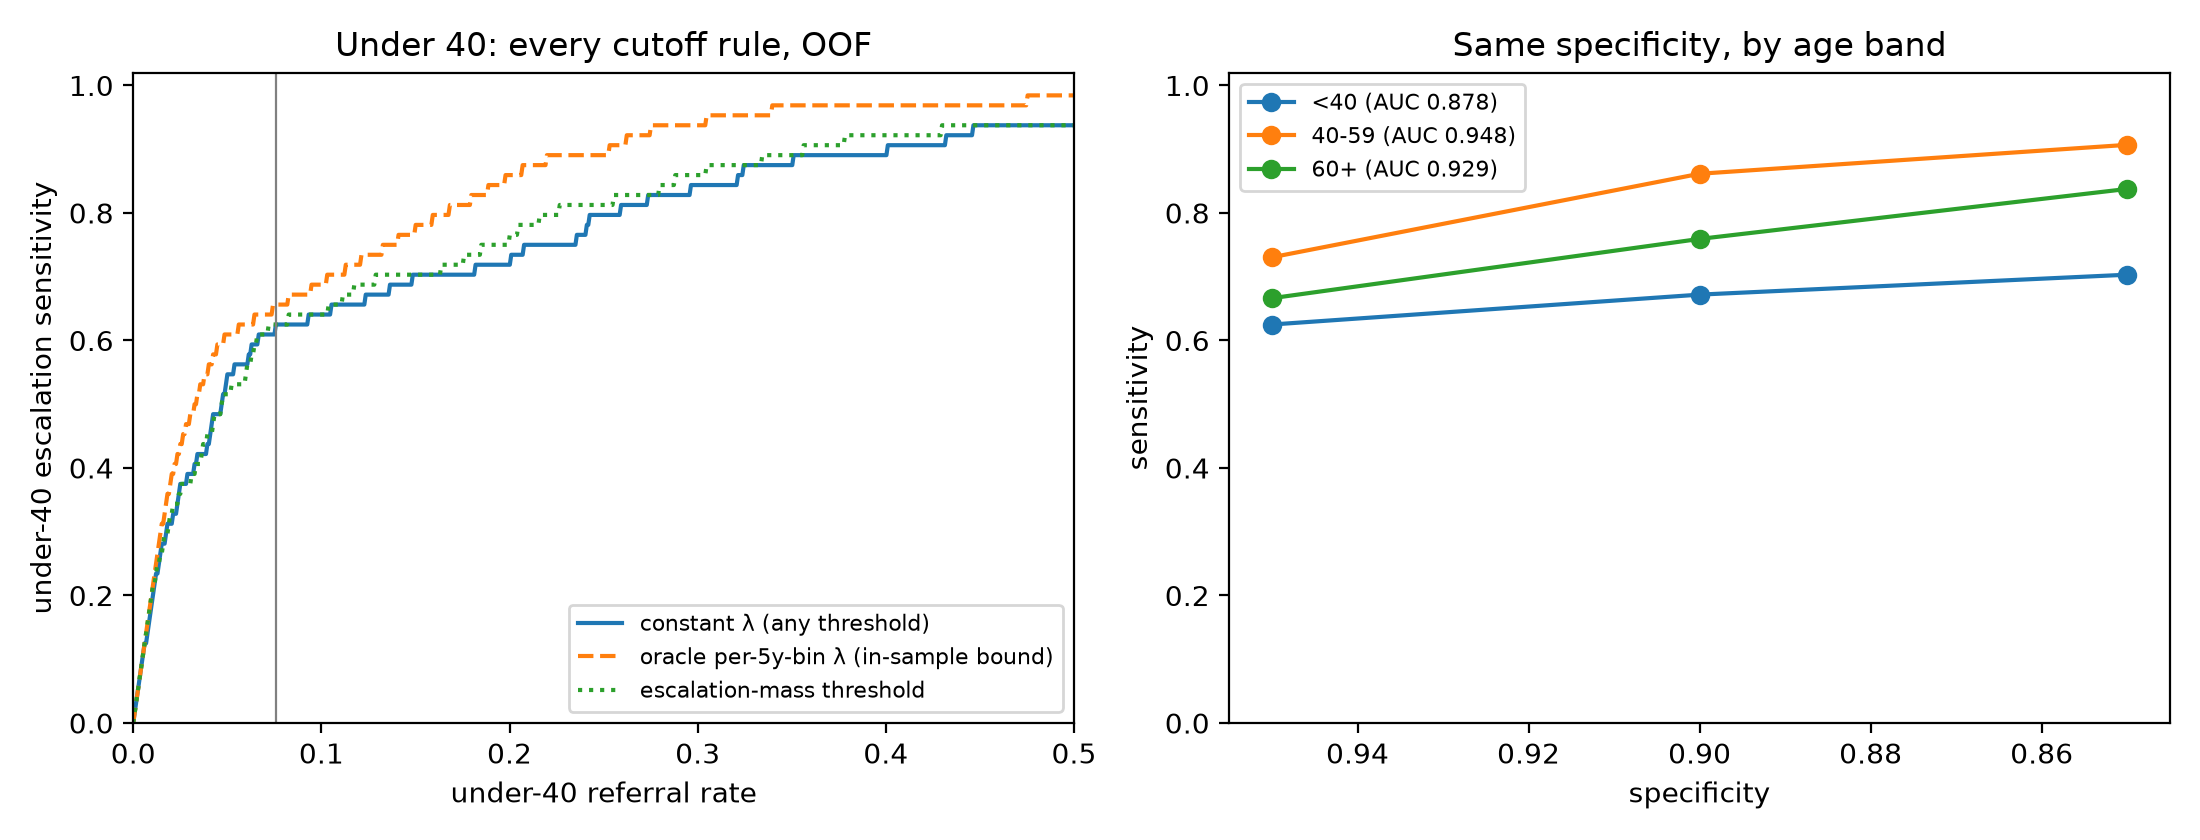
\includegraphics[width=\columnwidth]{under40_ceiling.png}
\caption{Left: \uforty{} sensitivity against \uforty{} referral for every cutoff rule on HAM
OOF predictions. The vertical line marks the frozen rule. Right: sensitivity at fixed
specificity, by age band.}
\label{fig:ceiling}
\end{figure}

\subsection{Nothing tested moves \uforty{} ranking}\label{sec:ranking}
Table~\ref{tab:ranking} lists every intervention aimed at the ranking.
\begin{itemize}
\item \emph{Frozen-feature probes} compared a dermatology foundation model \cite{yan2025panderm}
and DINOv2 \cite{oquab2024dinov2} with the in-repo ConvNeXt-Tiny trunk on the reserved cohort.
\item \emph{In-domain retraining} pooled all three archives. The composite recipe (384\,px plus
a class-balanced sampler) was compared with a pooled control, three seeds each, seed-matched.
\item \emph{Heads} were fit on frozen features.
\end{itemize}
No row reached its pre-registered target: $+0.05$, or $+0.03$ for the head probes, with an
interval excluding zero. Absolute \uforty{} partial AUCs on reserved sit in a narrow band: 0.720
to 0.750 for every retrained model, and 0.7335 for the deployed ensemble.

\begin{table}[t]
\caption{Interventions on \uforty{} ranking: $\Delta$ \uforty{} pAUC@0.20 [95\% CI].
\textsuperscript{\dag}Bonferroni-adjusted (three arms). Head probes used development rows; all other rows
used the reserved cohort.}
\label{tab:ranking}
\centering
\begin{tabular}{lr}
\toprule
Intervention (contrast) & $\Delta$ pAUC\\
\midrule
PanDerm ViT-B/16 $-$ ConvNeXt-Tiny & $-$0.036 [$-$0.083, 0.013]\\
DINOv2 ViT-B/14 $-$ ConvNeXt-Tiny & $-$0.073 [$-$0.118, $-$0.029]\\
Pooled 384\,px + sampler $-$ pooled control & 0.009 [$-$0.020, 0.037]\\
\quad same, best-epoch checkpoints & $-$0.011 [$-$0.037, 0.016]\\
Pooled refit head $-$ checkpoint head & 0.020 [$-$0.012, 0.054]\\
Domain-routed heads $-$ checkpoint head & 0.007 [$-$0.027, 0.040]\\
\uforty{} specialist head\textsuperscript{\dag} & $-$0.039 [$-$0.108, 0.034]\\
Hard-case reweighting\textsuperscript{\dag} & $-$0.000 [$-$0.013, 0.012]\\
Sex, site and age as inputs\textsuperscript{\dag} & 0.007 [$-$0.002, 0.017]\\
\bottomrule
\end{tabular}
\end{table}

In-domain training does help overall. The retrained composite beats the deployed ensemble by
0.180 [0.130, 0.225] in full-coverage Macro-F1 on the reserved cohort, but by only 0.004
[$-$0.052, 0.062] in \uforty{} partial AUC. This contrast is confounded by training corpus, and
we report it only as a deployment difference. Against the pooled control, the composite's
Macro-F1 difference depends on the checkpoint rule: $-$0.012 [$-$0.032, 0.010] with last-epoch
checkpoints and 0.032 [0.004, 0.056] with best-epoch checkpoints. We therefore claim neither.

\subsection{Decision layers reallocate referrals}\label{sec:decision}
Table~\ref{tab:decision} summarises the decision-layer sessions on the reserved cohort.

\begin{table}[t]
\caption{Decision layers on the reserved cohort: \uforty{} sensitivity gain [95\% CI] and the
\uforty{} workload it cost (abstention rows: referral rate; $\lambda$ rows: escalating-decision
rate; matched row: flag rate, escalated or referred).}
\label{tab:decision}
\centering
\begin{tabular}{lcc}
\toprule
Policy (comparator) & $\Delta$ sens. & Workload\\
\midrule
Per-band abstention (global), $R{=}0.20$ & 0.154 [0.104, 0.216] & 0.232$\to$0.454\\
Kernel $\lambda(\text{age})$ (frozen rule) & 0.208 [0.127, 0.296] & 0.145$\to$0.278\\
Per-hospital $\lambda$ (frozen rule), BCN & 0.216 [0.125, 0.313] & 0.160$\to$0.303\\
Combined policy (abstention), $R{=}0.20$ & 0.082 [0.042, 0.131] & 0.454$\to$0.608\\
Combined (matched abstention) & 0.004 [$-$0.014, 0.025] & 0.608 vs 0.558\\
\bottomrule
\end{tabular}
\end{table}

\emph{Per-band abstention} is the one positive result, and it cleared its MCID of 0.10. It works
by moving budget between bands:
\begin{itemize}
\item sensitivity in patients 60 and over fell by 0.100 [0.082, 0.118];
\item all-ages sensitivity fell by 0.040;
\item total referral fell slightly, by 0.017.
\end{itemize}
Neither the budget nor the floor transferred off HAM. A nominal 20\% budget referred 0.386 of
the reserved cohort. The nominal floor was met in none of 15 budget-by-band cells: 12 were
violated outright, and in 3 the point estimate fell below the floor while the interval still
reached it.

\emph{The age-resolved and per-hospital rules} both passed their primary endpoint and failed
their cost gates. Young-patient referral rose 1.92-fold and 1.90-fold, and \uforty{}
specificity fell from 0.960 to 0.857 and from 0.965 to 0.859 respectively. Neither gain came
from finer structure. The per-hospital fit selected full shrinkage, and pooled and per-hospital
$\lambda$ gave identical \uforty{} sensitivity. The gain was simply a larger \uforty{}
$\lambda$; on BCN it cost 1.95 extra referrals per extra catch.

\emph{The combined policy} (per-band calibration, then the age rule, then abstention) beat
abstention alone at equal nominal budget. At matched workload it did not: plain abstention
caught as many young patients with fewer \uforty{} flags. The per-band map also undid the frozen
\uforty{} $\lambda$, which had been fit under the global map. \uforty{} decision sensitivity
fell from 0.409 to 0.262.

\subsection{What does work, and what it does not touch}
\emph{Per-band calibration} removed the sign disagreement left by the global map. The spread of
the signed confidence gap across bands fell from 0.068 to 0.008, and \uforty{} ECE fell from
0.0276 to 0.0095. The spread of ECE across bands widened, from 0.015 to 0.021, and 60+ remained
the worst-calibrated band (0.0301). Calibration changed \uforty{} ranking by only 0.0072 in AUC.

\emph{A refit head on frozen features} raised reserved Macro-F1 from 0.419 to 0.534, about
63\% of the way to a retrained trunk. Routing to domain-specific heads added nothing over one
pooled head ($-$0.008 [$-$0.024, 0.007]). The out-of-scope gate rejected only 0.378 of
smartphone images from PAD-UFES-20 \cite{pacheco2020padufes}, and the three-way archive router
reached an accuracy of 0.932. Neither front-end component met its target.

\emph{Recipe screen.} On HAM validation, with three seeds, the fixed colour-constancy step
\cite{finlayson2004shades}, mixing augmentation, EMA with a longer schedule, a balanced sampler
and a metadata branch were all null against the control, whose seed standard deviation is
0.023. Resolution was the only lever: 384\,px gave $+$0.0297 (seed range 0.0097 to 0.0466). It was
already part of the retrained composite in Table~\ref{tab:ranking}.

\subsection{The deployed system and its contract}\label{sec:contract}
The adopted stack is the frozen ensemble with per-band abstention at $R{=}0.20$. Two further
layers were rejected at matched workload:
\begin{itemize}
\item the age rule, at $-$0.018 [$-$0.025, $-$0.011] all-ages sensitivity;
\item conformal sets \cite{angelopoulos2021raps} used as a referral trigger, at $-$0.069
[$-$0.086, $-$0.052].
\end{itemize}
The contract terms were issued on HAM data before the reserved read (Table~\ref{tab:contract}).
The plan declared failure as the expected outcome, and every term failed.

Against the ensemble at full coverage, the stack adds 0.301 [0.273, 0.328] system sensitivity
overall and 0.423 [0.310, 0.539] under 40, but it refers 0.386 of cases. Because the per-band
floor was not cleared, the gate for a third HAM test read stayed closed.

\begin{table}[t]
\caption{Contract of the deployed stack on the reserved cohort.}
\label{tab:contract}
\centering
\begin{tabular}{lcc}
\toprule
Term & Reserved [95\% CI] & Target\\
\midrule
System sens.\ $<$40 & 0.763 [0.655, 0.853] & $\ge$0.855\\
System sens.\ 40--59 & 0.704 [0.631, 0.771] & $\ge$0.855\\
System sens.\ 60+ & 0.674 [0.638, 0.713] & $\ge$0.855\\
Retained Macro-F1 & 0.465 [0.401, 0.516] & $\ge$0.888\\
Referral rate & 0.386 [0.363, 0.408] & $\le$0.250\\
NNB ($\pi{=}0.03$) & 13.6 & $\le$7.9\\
\bottomrule
\end{tabular}
\end{table}

% =====================================================================
\section{Discussion}
The two readings in the introduction are no longer equally plausible. If the argmax rule were
discarding a correct ranking, some decision layer should have raised \uforty{} sensitivity at
unchanged workload. None did. Every gain moved the operating point along the same ROC curve, and
that curve is lower for young patients. It stays lower on melanoma alone, across three
archives, across backbones and after in-domain training.

A decision layer is still useful. Per-band abstention lets a service choose who pays for
\uforty{} sensitivity, and our results price that choice: roughly a doubling of young-patient
referral, paid for by sensitivity in patients 60 and over. It should be presented as a
reallocation, with its cost beside it, and not as a fix.

The same evidence limits the claims of the deployed system. Budgets and floors fitted on HAM
over-refer on other archives, and the contract fails there. A deployment outside HAM-like
dermoscopy needs target-side recalibration before any floor is quoted.

% =====================================================================
\section{Limitations}\label{sec:limits}
\begin{itemize}
\item \emph{Reused evaluation set.} The reserved cohort was read 8 times under receipts, plus an
earlier unreceipted probe. The choice of which session ran next depended on earlier results, and
multiplicity across sessions is uncorrected. This weighs most on the positive results.
\item \emph{Demanding gates.} Some gates were hard to pass by construction. A 1.5-fold referral
cap fires for almost any sensitivity gain, and a $+$0.05 backbone margin is smaller than the
roughly 0.07 half-width of each backbone's interval. The matched-workload contrast is the cleaner evidence.
\item \emph{Truncated training.} Patience-based early stopping ended the pooled retraining runs
at 14 to 22 of 30 epochs. The claim that in-domain training does not lift \uforty{} ranking is
conditional on that recipe.
\item \emph{Pipeline defects found and fixed.} A defect in the colour-constancy step invalidated
the first screen of that arm. The re-run is null. The backbone probe's control used a bicubic
resize; under the deployed bilinear transform the control's \uforty{} partial AUC is 0.711. The
foundation-model contrast shrinks, but it still falls far short of its margin.
\item \emph{Endpoint form.} The first-declared endpoint was not read in exactly its declared form
(Sec.~\ref{sec:data}).
\item \emph{Deployed base.} The base is the HAM-only ensemble because the abstention thresholds
need cross-fitted predictions, which no retrained model has. A stack on a retrained base is
untested.
\item \emph{Skin tone.} Fitzpatrick evidence exists only for types I--IV. There is none for types
V and VI.
\end{itemize}

\section{Conclusion}
The \uforty{} melanoma blind spot in this dermoscopy triage system is a ranking limit. Decision
layers can move it between age bands at a measured price, but they cannot remove it. Closing the
gap needs more \uforty{} escalating lesions or a signal these images do not yet carry.

% =====================================================================
\begin{thebibliography}{99}

\bibitem{tschandl2018ham10000} P. Tschandl, C. Rosendahl, and H. Kittler, ``The HAM10000
dataset, a large collection of multi-source dermatoscopic images of common pigmented skin
lesions,'' \emph{Sci. Data}, vol. 5, 2018, Art. no. 180161.

\bibitem{codella2018isic} N. C. F. Codella \emph{et al.}, ``Skin lesion analysis toward
melanoma detection: A challenge at the 2017 International Symposium on Biomedical Imaging
(ISBI),'' in \emph{Proc. IEEE ISBI}, 2018, pp. 168--172.

\bibitem{combalia2019bcn20000} M. Combalia \emph{et al.}, ``BCN20000: Dermoscopic lesions in
the wild,'' 2019, \emph{arXiv:1908.02288}.

\bibitem{pacheco2020padufes} A. G. C. Pacheco \emph{et al.}, ``PAD-UFES-20: A skin lesion
dataset composed of patient data and clinical images collected from smartphones,'' \emph{Data
Brief}, vol. 32, 2020, Art. no. 106221.

\bibitem{liu2022convnext} Z. Liu \emph{et al.}, ``A ConvNet for the 2020s,'' in \emph{Proc.
IEEE/CVF CVPR}, 2022, pp. 11976--11986.

\bibitem{tan2019efficientnet} M. Tan and Q. V. Le, ``EfficientNet: Rethinking model scaling
for convolutional neural networks,'' in \emph{Proc. ICML}, 2019, pp. 6105--6114.

\bibitem{he2016resnet} K. He, X. Zhang, S. Ren, and J. Sun, ``Deep residual learning for
image recognition,'' in \emph{Proc. IEEE CVPR}, 2016, pp. 770--778.

\bibitem{huang2017densenet} G. Huang, Z. Liu, L. van der Maaten, and K. Q. Weinberger,
``Densely connected convolutional networks,'' in \emph{Proc. IEEE CVPR}, 2017, pp. 4700--4708.

\bibitem{kull2019dirichlet} M. Kull \emph{et al.}, ``Beyond temperature scaling: Obtaining
well-calibrated multi-class probabilities with Dirichlet calibration,'' in \emph{Proc.
NeurIPS}, 2019.

\bibitem{hebertjohnson2018multicalibration} \'{U}. H\'{e}bert-Johnson, M. P. Kim, O.
Reingold, and G. N. Rothblum, ``Multicalibration: Calibration for the
(computationally-identifiable) masses,'' in \emph{Proc. ICML}, 2018, pp. 1939--1948.

\bibitem{angelopoulos2024crc} A. N. Angelopoulos, S. Bates, A. Fisch, L. Lei, and T. Schuster,
``Conformal risk control,'' in \emph{Proc. ICLR}, 2024.

\bibitem{angelopoulos2021raps} A. N. Angelopoulos, S. Bates, M. Jordan, and J. Malik,
``Uncertainty sets for image classifiers using conformal prediction,'' in \emph{Proc. ICLR},
2021.

\bibitem{mcclish1989pauc} D. K. McClish, ``Analyzing a portion of the ROC curve,''
\emph{Med. Decis. Making}, vol. 9, no. 3, pp. 190--195, 1989.

\bibitem{clopper1934} C. J. Clopper and E. S. Pearson, ``The use of confidence or fiducial
limits illustrated in the case of the binomial,'' \emph{Biometrika}, vol. 26, no. 4,
pp. 404--413, 1934.

\bibitem{holm1979} S. Holm, ``A simple sequentially rejective multiple test procedure,''
\emph{Scand. J. Statist.}, vol. 6, no. 2, pp. 65--70, 1979.

\bibitem{yan2025panderm} S. Yan \emph{et al.}, ``A multimodal vision foundation model for
clinical dermatology,'' \emph{Nat. Med.}, 2025.

\bibitem{oquab2024dinov2} M. Oquab \emph{et al.}, ``DINOv2: Learning robust visual features
without supervision,'' \emph{Trans. Mach. Learn. Res.}, 2024.

\bibitem{finlayson2004shades} G. D. Finlayson and E. Trezzi, ``Shades of gray and colour
constancy,'' in \emph{Proc. IS\&T/SID Color Imaging Conf.}, 2004, pp. 37--41.

\end{thebibliography}

\end{document}
